\section{Produktumgebung}
Zur Beschreibung der Produktumgebung wird im Folgenden die Netzwerktopologie und ein Szenario betrachtet. Insbesondere werden auch die Voraussetzungen an Hardware und Software genauer beleuchtet.

\subsection{Szenario}
Abbildung 1 soll das im Folgenden geschilderte Szenario verbildlichen.

Wie bereits beschrieben, handelt es sich bei PECTO um ein Encryption-Framework, welches den effizienten und verschlüsselten Datenaustausch zwischen einzelnen \gloss{roten Netzen} durch ein \gloss{schwarzes Netz} ermöglicht.
Ein \gloss{rotes Netz} besteht aus einem physischen, durch Ethernet verbundenen Netzwerk, dass von einer Instanz des Systems geschützt wird.
Das \gloss{schwarze Netz} trennt mehrere verschiedene \gloss{rote Netze} voneinander.
Dabei agiert jede Instanz als Schnittstelle zwischen dem \gloss{schwarzen} und einem \gloss{roten Netz}.
Mehrere Instanzen bilden eine Gruppe, wenn sie die gleiche Netzgruppe schützen.
Eine Netzgruppe besteht dabei aus mehreren physisch getrennten \gloss{roten Netzen}, die logisch ein großes Netzwerk bilden.
Verschiedene Gruppen können zwar koexistieren, jedoch nicht miteinander kommunizieren.
Möchte nun eine Einheit aus einem roten Netz mit einer anderen aus einem zweiten roten Netz derselben Gruppe kommunizieren, werden die Daten an die für das Netz zuständige Instanz geleitet, welche Verschlüsselung und Weiterleitung übernimmt.
Kommt das Paket bei der anderen Instanz an, wird dieses, wie in den Zielbestimmungen beschrieben, klassifiziert und ggf. im dortigen roten Netz zur Zieladresse geschickt.     
 
  \begin{figure}  
    \begin{center}
	  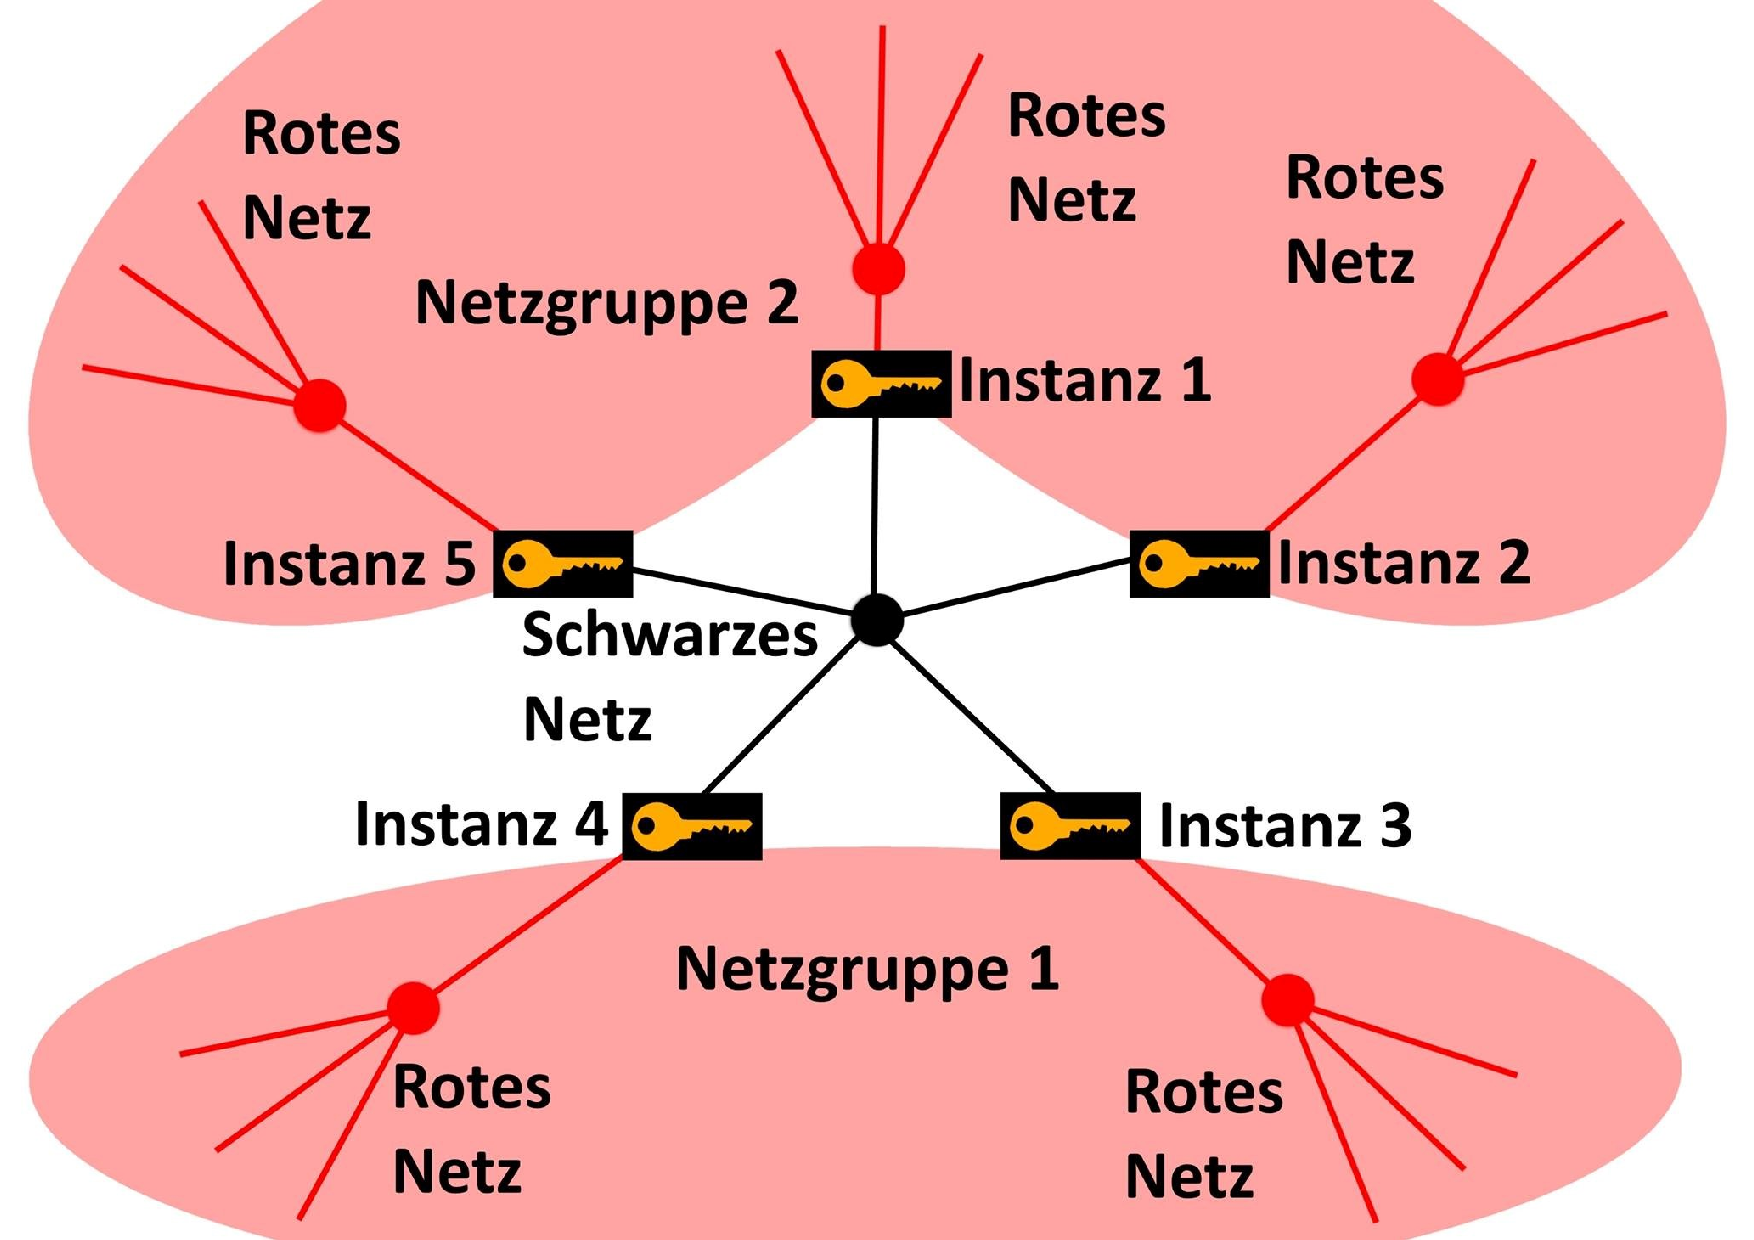
\includegraphics[width = 10cm]{Bilder/PECTO_Skizze.pdf}
	  \caption{Aufbau des Systems}
    \end{center}
  \end{figure}  
  
  
\subsection{Software}
Das System wird auf Linux-basierenden Bertriebssystemen lauffähig sein.

Eine Kerntechnologie, die genutzt wird um, die Anforderungen an dieses System angemessen umzusetzen, ist Intel's Data Plane Developement Kit (\gloss{DPDK}). 
Dieses Framework ermöglicht den direkten Zugriff aus dem Userspace auf die Netzwerkkarte. Es bietet zudem die Möglichkeit Pakete direkt in den Hauptspeicher des Rechners zu übertragen, ohne Interruptlast zu erzeugen. 
Für die erleichterte Bedienung wird eine Hardwareabstraktionsschicht (\gloss{EAL}) erzeugt, welche den Zugang auf Teile der Hardware des Linux-Kerns, durch Klassen, Methoden und Funktionen erlaubt.
Ein einfacherer Zugriff auf den Data-Link-Layer und Möglichkeiten zur schnellen Weiterleitung lassen sich durch erweiterbare Funktionen des Framework realisieren.
Zusätzliche hierzu bietet das \gloss{DPDK} auch noch eine Reihe von anderen Funktionen, welche für die Verschlüsselung, basierend auf \gloss{AES}, das Authentifizieren, dem Packet-Forwarding und der Schlüsselaushandlung genutzt werden.

\subsection{Hardware}

Das System soll Architekturen auf x64-Basis unterstützen. 
Um lauffähig zu sein, benötigt es außerdem \gloss{DPDK}-kompatible Netzwerkkarten und einen Prozessor, welcher die Nutzung von \gloss{AES-NI} möglich macht.
Zur Verwendung des Systems ist außerdem ein Zugang zu einem Ethernet-basierten Kommunikationskanal notwendig.
Dieser muss in der Lage sein, eine Übertragungsrate von bis zu 40 Gigabit/s zu realisieren.

\subsection{Netzwerktopologie}

Es gibt mehrere \gloss{rote Netze}, die zu einer Netzgruppe gehören, aber nicht direkt miteinander verbunden sind.
Alle Clients der Netzgruppe verwenden die gleiche Subnetzmaske.
Das \gloss{schwarze Netz} trennt die einzelnen \gloss{roten Netze}. 
Dabei ist die Topologie, welche im \gloss{schwarzen Netz} vorliegt, für das System unbedeutend.
Die Instanzen des Systems agieren lediglich als Übergang zwischen dem \gloss{schwarzen} und den \gloss{roten Netzen}.
Es wirkt nach außen hin wie ein \gloss{Layer-2-Switch}, welcher die Weiterleitung der Datenpakete auf dem Data-Link-Layer übernimmt. 







